% !TeX spellcheck = pl_PL
%%%%%%%%%%%%%%%%%%%%%%%%%%%%%%%%%%%%%%%%%%%
%                                        %
% Szablon pracy dyplomowej inzynierskiej %
% zgodny  z aktualnymi  przepisami  SZJK %
%                                        %
%%%%%%%%%%%%%%%%%%%%%%%%%%%%%%%%%%%%%%%%%%
%                                        %
%  (c) Krzysztof Simiński, 2018-2023     %
%                                        %
%%%%%%%%%%%%%%%%%%%%%%%%%%%%%%%%%%%%%%%%%%
%                                        %
% Najnowsza wersja szablonów jest        %
% podstępna pod adresem                  %
% github.com/ksiminski/polsl-aei-theses  %
%                                        %
%%%%%%%%%%%%%%%%%%%%%%%%%%%%%%%%%%%%%%%%%%
%
%
% Projekt LaTeXowy zapewnia odpowiednie formatowanie pracy,
% zgodnie z wymaganiami Systemu zapewniania jakości kształcenia.
% Proszę nie zmieniać ustawień formatowania (np. fontu,
% marginesów, wytłuszczeń, kursywy itd. ).
%
% Projekt można kompilować na kilka sposobów.
%
% 1. kompilacja pdfLaTeX
%
% pdflatex main
% bibtex   main
% pdflatex main
% pdflatex main
%
%
% 2. kompilacja XeLaTeX
%
% Kompilatacja przy użyciu XeLaTeXa różni się tym, że na stronie
% tytułowej używany jest font Calibri. Wymaga to jego uprzedniego
% zainstalowania.
%
% xelatex main
% bibtex  main
% xelatex main
% xelatex main
%
%
%%%%%%%%%%%%%%%%%%%%%%%%%%%%%%%%%%%%%%%%%%%%%%%%%%%%%
% W przypadku pytań, uwag, proszę pisać na adres:   %
%      krzysztof.siminski(małpa)polsl.pl            %
%%%%%%%%%%%%%%%%%%%%%%%%%%%%%%%%%%%%%%%%%%%%%%%%%%%%%
%
% Chcemy ulepszać szablony LaTeXowe prac dyplomowych.
% Wypełniając ankietę spod poniższego adresu pomogą
% Państwo nam to zrobić. Ankieta jest całkowicie
% anonimowa. Dziękujemy!


% https://docs.google.com/forms/d/e/1FAIpQLScyllVxNKzKFHfILDfdbwC-jvT8YL0RSTFs-s27UGw9CKn-fQ/viewform?usp=sf_link
%
%%%%%%%%%%%%%%%%%%%%%%%%%%%%%%%%%%%%%%%%%%%%%%%%%%%%%%%%%%%%%%%%%%%%%%%%%

%%%%%%%%%%%%%%%%%%%%%%%%%%%%%%%%%%%%%%%%%%%%%%%
%                                             %
% PERSONALIZACJA PRACY – DANE PRACY           %
%                                             %
%%%%%%%%%%%%%%%%%%%%%%%%%%%%%%%%%%%%%%%%%%%%%%%

% Proszę wpisać swoje dane w poniższych definicjach.

% TODO
% dane autora
\newcommand{\FirstNameAuthor}{Michał}
\newcommand{\SurnameAuthor}{Lubczyński}
\newcommand{\IdAuthor}{}   % numer albumu  (bez $\langle$ i $\rangle$)

% drugi autor:
%\newcommand{\FirstNameCoauthor}{Imię}   % Jeżeli jest drugi autor, to tutaj należy podać imię.
%\newcommand{\SurnameCoauthor}{Nazwisko} % Jeżeli jest drugi autor, to tutaj należy podać nazwisko.
%\newcommand{\IdCoauthor}{$\langle$wpisać właściwy$\rangle$}  % numer albumu drugiego autora (bez $\langle$ i $\rangle$)
% Gdy nie ma drugiego autora, należy zostawić poniższe definicje puste, jak poniżej. Gdy jest drugi autor, należy zakomentować te linie.
\newcommand{\FirstNameCoauthor}{Andrzej} % Jeżeli praca ma tylko jednego autora, to dane drugiego autora zostają puste.
\newcommand{\SurnameCoauthor}{Zagórski}   % Jeżeli praca ma tylko jednego autora, to dane drugiego autora zostają puste.
\newcommand{\IdCoauthor}{}  % Jeżeli praca ma tylko jednego autora, to dane drugiego autora zostają puste.
%%%%%%%%%%
\newcommand{\FirstNameCoXauthor}{Eryk} % Jeżeli praca ma tylko jednego autora, to dane drugiego autora zostają puste.
\newcommand{\SurnameCoXauthor}{SZMYT}   % Jeżeli praca ma tylko jednego autora, to dane drugiego autora zostają puste.
\newcommand{\IdCoCoauthor}{}  % Jeżeli praca ma tylko jednego autora, to dane drugiego autora zostają puste.

\newcommand{\Supervisor}{Dr. Inż. Aleksander Iwaniak}     % dane promotora (bez $\langle$ i $\rangle$)
\newcommand{\Title}{Framer - Wizualizacja danych z kamery termowizyjnej}           % tytuł pracy po polsku
\newcommand{\TitleAlt}{Framer - Thermal Camera Data Visualizatioh}                     % thesis title in English
\newcommand{\Program}{}            % kierunek studiów  (bez $\langle$ i $\rangle$)
\newcommand{\Specialisation}{}     % specjalność  (bez $\langle$ i $\rangle$)
\newcommand{\Departament}{}        % katedra promotora  (bez $\langle$ i $\rangle$)

% Jeżeli został wyznaczony promotor pomocniczy lub opiekun, proszę go/ją wpisać ...
\newcommand{\Consultant}{} % dane promotora pomocniczego, opiekuna (bez $\langle$ i $\rangle$)
% ... w przeciwnym razie proszę zostawić puste miejsce jak poniżej:
%\newcommand{\Consultant}{} % brak promotowa pomocniczego / opiekuna

% koniec fragmentu do modyfikacji
%%%%%%%%%%%%%%%%%%%%%%%%%%%%%%%%%%%%%%%%%%


%%%%%%%%%%%%%%%%%%%%%%%%%%%%%%%%%%%%%%%%%%%%%%%
%                                             %
% KONIEC PERSONALIZACJI PRACY                 %
%                                             %
%%%%%%%%%%%%%%%%%%%%%%%%%%%%%%%%%%%%%%%%%%%%%%%

%%%%%%%%%%%%%%%%%%%%%%%%%%%%%%%%%%%%%%%%


%%%%%%%%%%%%%%%%%%%%%%%%%%%%%%%%%%%%%%%%%%%%%%%
%                                             %
% PROSZĘ NIE MODYFIKOWAĆ PONIŻSZYCH USTAWIEŃ! %
%                                             %
%%%%%%%%%%%%%%%%%%%%%%%%%%%%%%%%%%%%%%%%%%%%%%%



\documentclass[a4paper,twoside,12pt]{book}
\usepackage[utf8]{inputenc}                                      
\usepackage[T1]{fontenc}  
\usepackage{amsmath,amsfonts,amssymb,amsthm}
\usepackage[british,polish]{babel} 
\usepackage{indentfirst}
\usepackage{xurl}
\usepackage{xstring}
\usepackage{ifthen}



\usepackage{ifxetex}

\ifxetex
	\usepackage{fontspec}
	\defaultfontfeatures{Mapping=tex—text} % to support TeX conventions like ``——-''
	\usepackage{xunicode} % Unicode support for LaTeX character names (accents, European chars, etc)
	\usepackage{xltxtra} % Extra customizations for XeLaTeX
\else
	\usepackage{lmodern}
\fi



\usepackage[margin=2.5cm]{geometry}
\usepackage{graphicx} 
\usepackage{hyperref}
\usepackage{booktabs}
\usepackage{tikz}
\usepackage{pgfplots}
\usepackage{mathtools}
\usepackage{geometry}
\usepackage{subcaption}   % subfigures
\usepackage[page]{appendix} % toc,
\renewcommand{\appendixtocname}{Dodatki}
\renewcommand{\appendixpagename}{Dodatki}
\renewcommand{\appendixname}{Dodatek}

\usepackage{csquotes}
\usepackage[natbib=true,backend=bibtex,maxbibnames=99]{biblatex}  % kompilacja bibliografii BibTeXem
%\usepackage[natbib=true,backend=biber,maxbibnames=99]{biblatex}  % kompilacja bibliografii Biberem
\bibliography{biblio}

\usepackage{ifmtarg}   % empty commands  

\usepackage{setspace}
\onehalfspacing


\frenchspacing



%%%% TODO LIST GENERATOR %%%%%%%%%

\usepackage{color}
\definecolor{brickred}      {cmyk}{0   , 0.89, 0.94, 0.28}

\makeatletter \newcommand \kslistofremarks{\section*{Uwagi} \@starttoc{rks}}
  \newcommand\l@uwagas[2]
    {\par\noindent \textbf{#2:} %\parbox{10cm}
{#1}\par} \makeatother


\newcommand{\ksremark}[1]{%
{%\marginpar{\textdbend}
{\color{brickred}{[#1]}}}%
\addcontentsline{rks}{uwagas}{\protect{#1}}%
}

\newcommand{\comma}{\ksremark{przecinek}}
\newcommand{\nocomma}{\ksremark{bez przecinka}}
\newcommand{\styl}{\ksremark{styl}}
\newcommand{\ortografia}{\ksremark{ortografia}}
\newcommand{\fleksja}{\ksremark{fleksja}}
\newcommand{\pauza}{\ksremark{pauza `--', nie dywiz `-'}}
\newcommand{\kolokwializm}{\ksremark{kolokwializm}}
\newcommand{\cudzyslowy}{\ksremark{,,polskie cudzysłowy''}}

%%%%%%%%%%%%%% END OF TODO LIST GENERATOR %%%%%%%%%%%

\newcommand{\printCoauthor}{%		
    \StrLen{\FirstNameCoauthor}[\FNCoALen]
    \ifthenelse{\FNCoALen > 0}%
    {%
		{\large\bfseries\Coauthor\par}
	
		{\normalsize\bfseries \LeftId \IdCoauthor\par}
		\vspace{2mm}

		{\large\bfseries\FirstNameCoXauthor\space \SurnameCoXauthor}
	

    }%
    {}
} 

%%%%%%%%%%%%%%%%%%%%%
\newcommand{\autor}{%		
    \StrLen{\FirstNameCoauthor}[\FNCoALenXX]
    \ifthenelse{\FNCoALenXX > 0}%
    {\Title}%
	{\FirstNameAuthor\ \SurnameAuthor}%
}
%%%%%%%%%%%%%%%%%%%%%

\StrLen{\FirstNameCoauthor}[\FNCoALen]
\ifthenelse{\FNCoALen > 0}%
{%
\author{\FirstNameAuthor\ \SurnameAuthor, \FirstNameCoauthor\ \SurnameCoauthor}
}%
{%
\author{\FirstNameAuthor\ \SurnameAuthor}
}%

%%%%%%%%%%%% ZYWA PAGINA %%%%%%%%%%%%%%%
% brak kapitalizacji zywej paginy
\usepackage{fancyhdr}
\pagestyle{fancy}
\fancyhf{}
\fancyhead[LO]{\nouppercase{\it\rightmark}}
\fancyhead[RE]{\nouppercase{\it\leftmark}}
\fancyhead[LE,RO]{\it\thepage}


\fancypagestyle{tylkoNumeryStron}{%
   \fancyhf{} 
   \fancyhead[LE,RO]{\it\thepage}
}

\fancypagestyle{bezNumeracji}{%
   \fancyhf{} 
   \fancyhead[LE,RO]{}
}


\fancypagestyle{NumeryStronNazwyRozdzialow}{%
   \fancyhf{} 
   \fancyhead[LE]{\nouppercase{\autor}}
   \fancyhead[RO]{\nouppercase{\leftmark}} 
   \fancyfoot[CE, CO]{\thepage}
}


%%%%%%%%%%%%% OBCE WTRETY  
\newcommand{\obcy}[1]{\emph{#1}}
\newcommand{\english}[1]{{\selectlanguage{british}\obcy{#1}}}
%%%%%%%%%%%%%%%%%%%%%%%%%%%%%

% polskie oznaczenia funkcji matematycznych
\renewcommand{\tan}{\operatorname {tg}}
\renewcommand{\log}{\operatorname {lg}}

% jeszcze jakies drobiazgi

\newcounter{stronyPozaNumeracja}

%%%%%%%%%%%%%%%%%%%%%%%%%%% 
\newcommand{\printOpiekun}[1]{%		

    \StrLen{\Consultant}[\mystringlen]
    \ifthenelse{\mystringlen > 0}%
    {%
       {\large{\bfseries OPIEKUN, PROMOTOR POMOCNICZY}\par}
       
       {\large{\bfseries \Consultant}\par}
    }%
    {}
} 
%
%%%%%%%%%%%%%%%%%%%%%%%%%%%%%%%%%%%%%%%%%%%%%%
 
% Proszę nie modyfikować poniższych definicji!
\newcommand{\Author}{\FirstNameAuthor\ \MakeUppercase{\SurnameAuthor}} 
\newcommand{\Coauthor}{\FirstNameCoauthor\ \MakeUppercase{\SurnameCoauthor}}
\newcommand{\Type}{Dokumentacja do Project Basic Learning}
\newcommand{\Faculty}{Wydział Inzynierii Materialoweji} 
\newcommand{\Polsl}{Politechnika Śląska}
\newcommand{\Logo}{politechnika_sl_logo_bw_pion_pl.pdf}
\newcommand{\LeftId}{}
\newcommand{\LeftProgram}{}
\newcommand{\LeftSpecialisation}{}
\newcommand{\LeftSUPERVISOR}{PROWADZĄCY PRACĘ}
\newcommand{\LeftDEPARTMENT}{KATEDRA}
%%%%%%%%%%%%%%%%%%%%%%%%%%%%%%%%%%%%%%%%%%%%%%

%%%%%%%%%%%%%%%%%%%%%%%%%%%%%%%%%%%%%%%%%%%%%%%
%                                             %
% KONIEC USTAWIEŃ                             %
%                                             %
%%%%%%%%%%%%%%%%%%%%%%%%%%%%%%%%%%%%%%%%%%%%%%%




%%%%%%%%%%%%%%%%%%%%%%%%%%%%%%%%%%%%%%%%%%%%%%%
%                                             %
% MOJE PAKIETY, USTAWIENIA ITD                %
%                                             %
%%%%%%%%%%%%%%%%%%%%%%%%%%%%%%%%%%%%%%%%%%%%%%%

% Tutaj proszę umieszczać swoje pakiety, makra, ustawienia itd.


 
%%%%%%%%%%%%%%%%%%%%%%%%%%%%%%%%%%%%%%%%%%%%%%%%%%%%%%%%%%%%%%%%%%%%%
% listingi i fragmentu kodu źródłowego 
% pakiet: listings lub minted
% % % % % % % % % % % % % % % % % % % % % % % % % % % % % % % % % % % 

% biblioteka listings
\usepackage{listings}
\lstset{%
morekeywords={string,exception,std,vector},% słowa kluczowe rozpoznawane przez pakiet listings
language=C++,% C, Matlab, Python, SQL, TeX, XML, bash, ... – vide https://www.ctan.org/pkg/listings
commentstyle=\textit,%
identifierstyle=\textsf,%
keywordstyle=\sffamily\bfseries, %\texttt, %
%captionpos=b,%
tabsize=3,%
frame=lines,%
numbers=left,%
numberstyle=\tiny,%
numbersep=5pt,%
breaklines=true,%
escapeinside={@*}{*@},%
}

% % % % % % % % % % % % % % % % % % % % % % % % % % % % % % % % % % % 
% pakiet minted
%\usepackage{minted}

% pakiet wymaga specjalnego kompilowania:
% pdflatex -shell-escape main.tex
% xelatex  -shell-escape main.tex

%\usepackage[chapter]{minted} % [section]
%%\usemintedstyle{bw}   % czarno-białe kody 
%
%\setminted % https://ctan.org/pkg/minted
%{
%%fontsize=\normalsize,%\footnotesize,
%%captionpos=b,%
%tabsize=3,%
%frame=lines,%
%framesep=2mm,
%numbers=left,%
%numbersep=5pt,%
%breaklines=true,%
%escapeinside=@@,%
%}

%%%%%%%%%%%%%%%%%%%%%%%%%%%%%%%%%%%%%%%%%%%%%%%%%%%%%%%%%%%%%%%%%%%%%



%%%%%%%%%%%%%%%%%%%%%%%%%%%%%%%%%%%%%%%%%%%%%%%
%                                             %
% KONIEC MOICH USTAWIEŃ                       %
%                                             %
%%%%%%%%%%%%%%%%%%%%%%%%%%%%%%%%%%%%%%%%%%%%%%%



%%%%%%%%%%%%%%%%%%%%%%%%%%%%%%%%%%%%%%%%


\begin{document}
%\kslistofremarks

\frontmatter

%%%%%%%%%%%%%%%%%%%%%%%%%%%%%%%%%%%%%%%%%%%%%%%
%                                             %
% PROSZĘ NIE MODYFIKOWAĆ STRONY TYTUŁOWEJ!    %
%                                             %
%%%%%%%%%%%%%%%%%%%%%%%%%%%%%%%%%%%%%%%%%%%%%%%


%%%%%%%%%%%%%%%%%%  STRONA TYTUŁOWA %%%%%%%%%%%%%%%%%%%
\pagestyle{empty}
{
	\newgeometry{top=1.5cm,%
	             bottom=2.5cm,%
	             left=3cm,
	             right=2.5cm}
 
	\ifxetex 
	  \begingroup
	  \setsansfont{Calibri}
	   
	\fi 
	 \sffamily
	\begin{center}
	\includegraphics[width=50mm]{\Logo}
	 
	
	{\Large\bfseries\Type\par}
	
	\vfill  \vfill  
			 
	{\large\Title\par}
	
	\vfill  
		
	{\large\bfseries\Author\par}

	{\normalsize\bfseries \LeftId \IdAuthor}

	\printCoauthor
	
	\vfill  		
 
	{\large{\bfseries \LeftProgram} \Program\par} 
	
	{\large{\bfseries \LeftSpecialisation} \Specialisation\par} 
	 		
	\vfill  \vfill 	\vfill 	\vfill 	\vfill 	\vfill 	\vfill  
	 
	{\large{\bfseries \LeftSUPERVISOR}\par}
	
	{\large{\bfseries \Supervisor}\par}
				
	{\large{\bfseries \LeftDEPARTMENT\ \Departament} \par}
		
	{\large{\bfseries \Faculty}\par}
		
	\vfill  \vfill  

    	
    \printOpiekun{\Consultant}
    
	\vfill  \vfill  
		
    {\large\bfseries  Katowice \the\year}

   \end{center}	
       \ifxetex 
       	  \endgroup
       \fi
	\restoregeometry
}
  
%%%%%%%%%%%%%%%%%%%%%%%%%%%%%%%%%%%%%%%%%%%%%%%
%                                             %
% KONIEC STRONY TYTUŁOWEJ                     %
%                                             %
%%%%%%%%%%%%%%%%%%%%%%%%%%%%%%%%%%%%%%%%%%%%%%%  


\cleardoublepage

\rmfamily\normalfont
\pagestyle{empty}


%%% No to zaczynamy pisać pracę :-) %%%%

% TODO
\subsubsection*{Tytuł pracy} 
\Title

\subsubsection*{Streszczenie}  
Framer.py to aplikacja w języku Python, która wizualizuje dane z kamery termowizyjnej MLX90640 podłączonej do Raspberry Pi 4B za pośrednictwem magistrali I2C. Aplikacja wykorzystuje SocketIO, biblioteki Adafruit i Flask, aby zapewnić interaktywne pomiary i dane w czasie rzeczywistym. Przeglądaj i analizuj rozkłady temperatur w przyjaznej dla użytkownika kanwie HTML.

\subsubsection*{Słowa kluczowe} 
Raspberry, Termowizja, MLX90640, Python, HTML, Canvas

\subsubsection*{Thesis title} 
\begin{otherlanguage}{british}
\TitleAlt

\end{otherlanguage}

\subsubsection*{Abstract} 
\begin{otherlanguage}{british}
Framer.py is a Python application that visualizes thermal camera data from the MLX90640 model connected to a Raspberry Pi 4B via the I2C bus. The application utilizes SocketIO, Adafruit libraries, and Flask to provide a real-time interactive experience. Explore and analyze temperature distributions in a user-friendly HTML canvas.
\end{otherlanguage}
\subsubsection*{Key words}  
\begin{otherlanguage}{british}
Raspberry, Thermo-vision, MLX90640, Python, HTML, Canvas
\end{otherlanguage}




%%%%%%%%%%%%%%%%%% SPIS TRESCI %%%%%%%%%%%%%%%%%%%%%%
% Add \thispagestyle{empty} to the toc file (main.toc), because \pagestyle{empty} doesn't work if the TOC has multiple pages
\addtocontents{toc}{\protect\thispagestyle{empty}}
\tableofcontents

%%%%%%%%%%%%%%%%%%%%%%%%%%%%%%%%%%%%%%%%%%%%%%%%%%%%%
\setcounter{stronyPozaNumeracja}{\value{page}}
\mainmatter
\pagestyle{empty}

\cleardoublepage

\pagestyle{NumeryStronNazwyRozdzialow}

%%%%%%%%%%%%%% wlasciwa tresc pracy %%%%%%%%%%%%%%%%%

% TODO
\chapter{Wstęp}
\label{ch:wstep}





Celem pracy jest stworzenie oprogramowania do przechwytywania danych z modulu kamery termowizyjnej - model MLX 90640. Do tego celu wykorzystano Raspberry Pi 4b do którego podłączono za pomocą przewodów połączeniowych "I2C/UART - 4-pinowy wtyk żeński", moduł kamery wspomniany wcześniej z kątem widzenia 110°, komunikujący się poprzez włączony w systemie Ubuntu, interfejs I2C. Matryca kamery 32x24 umożliwia pomiar temperatury w zakresie od -40°C do 300°C z dużą dokładnością do 1,5°C. Płytka kamery zasilana jest napięciem 3,3 V ale umożliwia także podpięcie pod 5V. Częstotliwość odświeżania zostala ustawiona na 2Hz. Program framer.py na platforme raspberry został napisany z myślą o przedstawianiu zjawisk termicznych obserwowanych za pomocą mobilnego stanowiska kierowanego przez prowadzącego. Umożliwia klientom w sieci lokalnej do obserwacji w czasie rzeczywistym zjawisk które mogą wykonywać się także w znacznej odległości od nich za pomocą dowolnego urządzenia z dostępem do sieci w której znajduje się aparat do badania termicznego. Administrator sieci lokalnej, którym w założeniach jest prowadzący zajęcia i nadzorujący obserwacje, ma prawo wpuszczenia konkretnych hostów co jednoznacznie daje im prawo do korzystania z uruchomionej aplikacji na urządzeniu do przechwytywania obrazu. Klienci mają dostęp do:
\begin{itemize}
\item Zmiany mapy kolorów za pomocą pola wyboru w celu lepszej interpretacji danych.
\item Wyświetlanie temperatury pod kursorem myszy w celu uzyskania natychmiastowej informacji zwrotnej
\item Śledzenie najgorętszego miejsca wraz z jego temperatura wypisaną w kolorze widocznym na tle.
\item Śledzenie temperatury w określonym punkcie kanwy
\item Skala temperatury dynamicznie aktualizowana po prawej stronie obszaru roboczego.
\item Przechwytywanie obrazu .png rzeczywistych danych wraz z skalą i każdym znacznikiem który śledzimy.
\item Nagrywanie wideo reagujące na start/stop przez maksymalnie 10 minut w najwyższej możliwej jakości 2 FPS
\item Nagrywanie poklatkowe z możliwością wyboru liczby klatek na sekundę.
\item Zapisywanie w lokalnych plikach hosta z dokładną datą i godziną przechwycenia.
\end{itemize}
\begin{figure}[h]
  \centering
  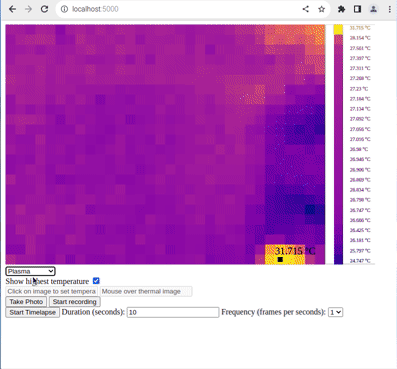
\includegraphics[width=0.8\textwidth]{frame_014_delay-0.1s.png}
  \caption{Interfejs użytkownika}
  \label{fig:obrazek}
\end{figure}









% TODO
\chapter{Ustawienia dla prowadzącego}
\label{ch:Ustawienia-dla-prowadzacego}
Aby aplikacja została uruchomiona w środowisku przygotowanym przez jednegp z współtwórców, wystarczy po uruchomieniu systemu, upewnić się o wystąpieniu zielonej sygnalizacji przez diodę led, na module kamery potwierdzające poprawne podłączenie jej do zasilania. Następnie należy upewnić się o poprawnym połączeniu z modułem poprzez polecenie: \lstinline| i2cdetect -y 1|. Jeżeli wystąpi problem z uruchomieniem polecenia należy doinstalować brakującą bibliotekę poleceniem: \lstinline|sudo apt-get install i2c-tools|. Jeżeli po pomyślnym wykonaniu pierwszej komendy, występuje zapis 33 mamy potwierdzenie o poprawnej komunikacji mikrokontrolera przez interfejs i2c z kamerą. W terminalu należy wywołać wówczas za pomoca polecenia python program z sciezka o ile nie znajdujemy sie w jego lokalizacji. Przykładowe polecenie może wyglądać: \lstinline| python3 Desktop\Framer\framer.py|

Aby aplikacja została uruchomiona w nowym środowisku tj Raspberry z kamerą MLX90640, wystarczające powinno być skopiowanie repozytorium pod adresem \lstinline|github.com/michalubczynski/Framer|. W przypadku braku dostępu do sieci, niezbędne biblioteki to kolejno:
\begin{itemize}
\item adafruit-circuitpython-mlx90640
\item flask
\item python-socketio
\end{itemize}
W przypadku braku dostępu do repozytorium lecz posiadając dostęp do sieci, należy wprowadzić w terminalu następujące polecenia:
\newline
\lstinline|pip install adafruit-circuitpython-mlx90640 flask python-socketio|
\newline
\lstinline|python3 framer.py|







 Częstotliwość odświeżania zadeklarowana przez producenta 0,5 Hz do 64 Hz po przeprowadzonych testach została zdementowana albowiem wartosci powyzej 2Hz wpływały wyłącznie negatywnie na czas odświeżania klatek.
Aby klienci mogli korzystać z danych rozpropagowywanych przez mikrokontroler, musi zostać na nim uruchomiona aplikacja 
Aby nieprzerwanie przechwytywac obraz z wybranymi ustawieniami jak i podczas jakichkolwiek operacji klient jak i operator zobowiazani sa do zapewnienia stałego, stosunkowo szybkiego łącza internetowego jeśli mówimy o sieci lokalnej z wieloma instancjami klientow. Dla samodzielnej aplikacji na aparacie nie jest wymagane polaczenie z internetem. Połączenie następuje poprzez 



% TODO
\chapter{Ustawienia dla klienta}
\label{ch:Ustawienia-dla-klienta}
Dostęp do aplikacji uzyskujemy poprzez wprowadzenie w przeglądarce IPaparatu::5000 co jest kolejno adresem ip aparatu, o ktory należy zapytać operatora, oraz port na ktorym hostowana aplikacja.
Nie zostały przetestowane maksymalne ilości jednocześnie korzystających hostów z portu z dostępem do aplikacji.







% TODO
\chapter{Ograniczenia aplikacji}
\label{ograniczenia-aplikacji}


\begin{itemize}
\item Przegladarki 
\item Ilosc klientow
\item Odswiezanie
\item UDP a nie TCP
\item Interpolacja obrazu a wypelnionej canvy
\end{itemize}


% TODO
\chapter{Problemy podczas developmentu}
\label{problems}


\begin{itemize}
\item Zrzuty ekranu i gify
\item Poszukiwania biblioteki do zapisu wideo i kodeki

\end{itemize}


% TODO
\chapter{Podsumowanie i wnioski}
\begin{itemize}
\item uzyskane wyniki w świetle postawionych celów i zdefiniowanych wyżej wymagań
\item kierunki ewentualnych danych prac (rozbudowa funkcjonalna …)
\item problemy napotkane w trakcie pracy
\end{itemize}



\backmatter




\end{document}




